\chapter{Implementation}


\section{Implementation Plan \textit{for Sem – 8}}
Implementation Plan for the Sem - 8 to include the following:\\
Gantt chart
\begin{figure}[h]
	\centering
    \hfill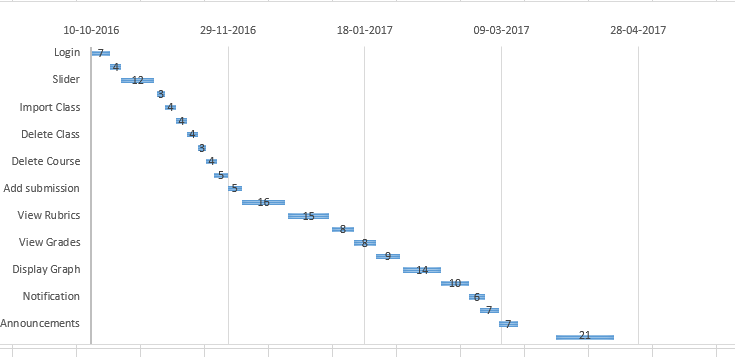
\includegraphics[scale=.85,angle=360]{project/images/Capture}\hspace{\fill}
    \caption{Gantt chart}
\end{figure}\\
\newpage
Work Break down structure \\ 
\begin{figure}[h]
	\centering
    \hfill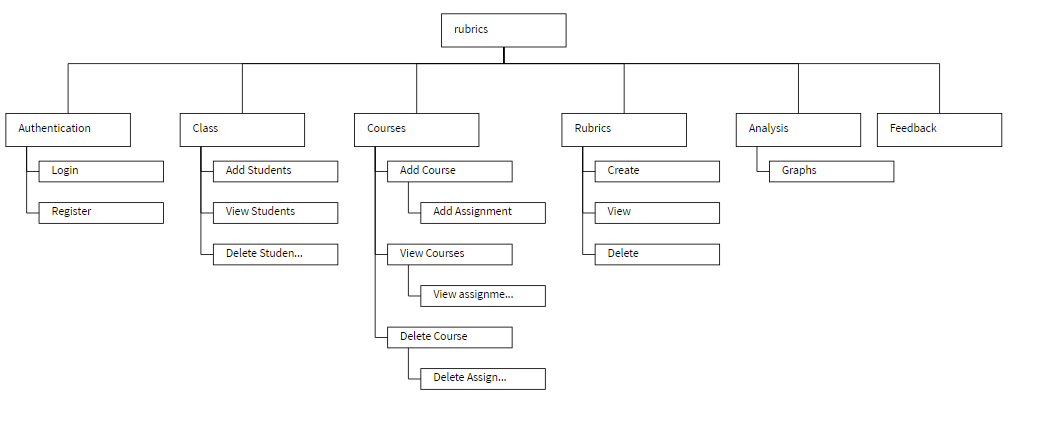
\includegraphics[scale=.60,angle=360]{project/images/wbs}\hspace{\fill}
    \caption{WBS chart}
\end{figure}\\

\section{Android and Web Application GUI}
\subsection{Android GUI}
\begin{figure}[!h]
\begin{minipage}[t]{0.5\linewidth}
    \centering
\hfill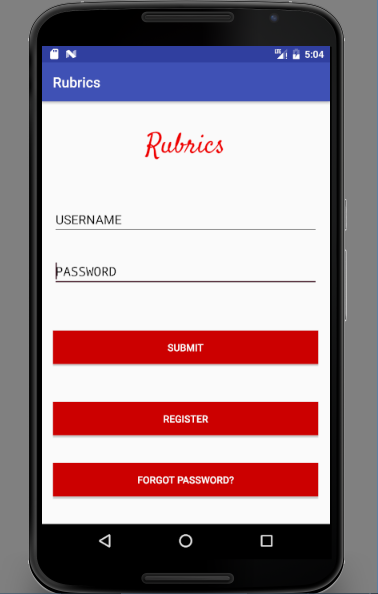
\includegraphics[scale=.65]{project/images/loginnew}\hspace*{\fill}
    \caption{Login Page}
    \label{f1}
\end{minipage}
\hspace{0.1cm}
\begin{minipage}[t]{0.5\linewidth} 
    \centering
\hfill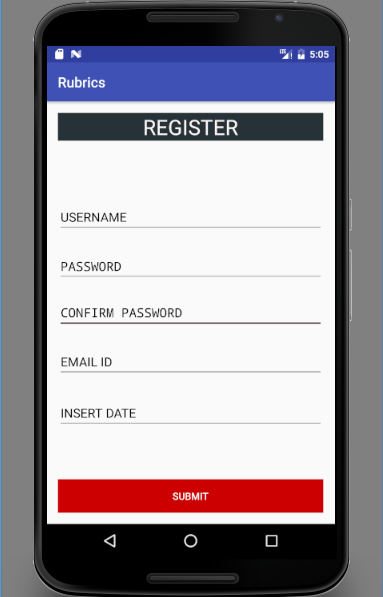
\includegraphics[scale=.65]{project/images/registernew}\hspace*{\fill}
    \caption{Registration Page}
    \label{f2}
\end{minipage}        
\end{figure}  

\begin{figure}[!h]
\begin{minipage}[t]{0.5\linewidth}
    \centering
\hfill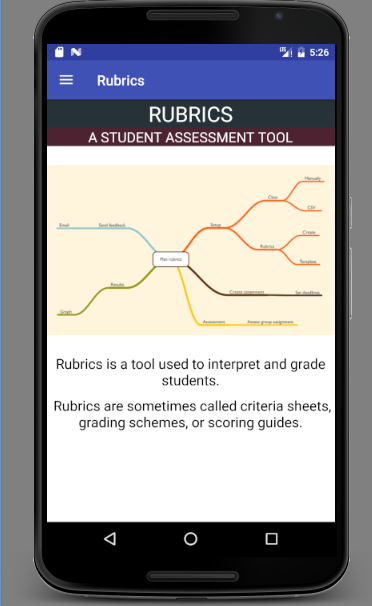
\includegraphics[scale=.65]{project/images/welcomepage}\hspace*{\fill}
    \caption{Quick Overview}
    \label{f1}
\end{minipage}
\hspace{0.1cm}
\begin{minipage}[t]{0.5\linewidth} 
    \centering
\hfill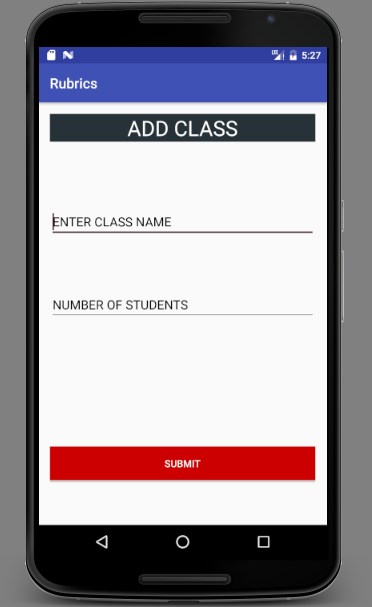
\includegraphics[scale=.65]{project/images/manageclassnew}\hspace*{\fill}
    \caption{Manage Class Page}
    \label{f2}
\end{minipage}        
\end{figure}  

\begin{figure}[!h]
\begin{minipage}[t]{0.5\linewidth}
    \centering
\hfill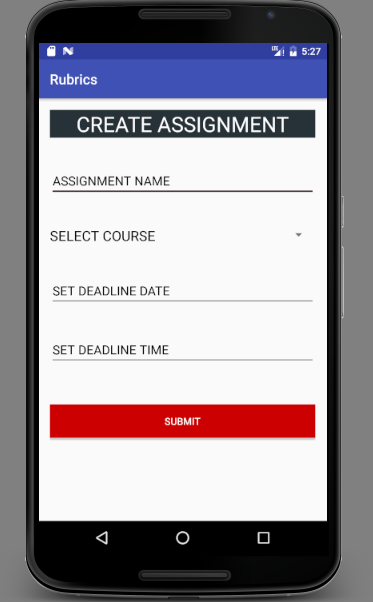
\includegraphics[scale=.65]{project/images/createassigmentnew}\hspace*{\fill}
    \caption{Create Asssignment}
    \label{f1}
\end{minipage}
\hspace{0.1cm}
\begin{minipage}[t]{0.5\linewidth} 
    \centering
\hfill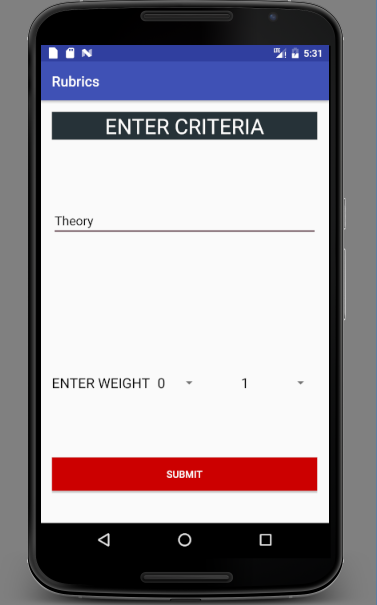
\includegraphics[scale=.65]{project/images/createrubricnew}\hspace*{\fill}
    \caption{Create Rubrics}
    \label{f2}
\end{minipage}        
\end{figure}  

\begin{figure}[!h]
\begin{minipage}[t]{0.5\linewidth}
    \centering
\hfill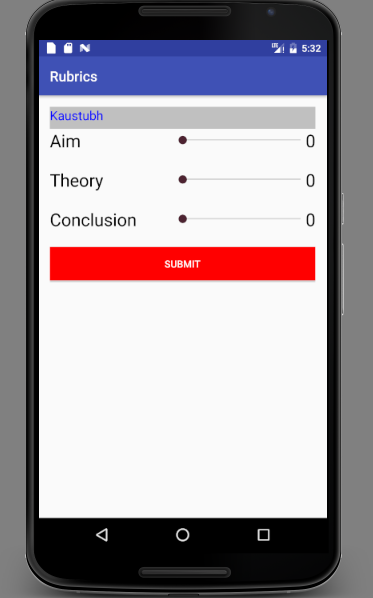
\includegraphics[scale=.65]{project/images/gradingnew}\hspace*{\fill}
    \caption{Start Grading}
    \label{f1}
\end{minipage}        
\end{figure}  

\subsection{Web GUI}
\begin{figure}[H]
\begin{minipage}[t]{0.5\linewidth}
    \centering
\hfill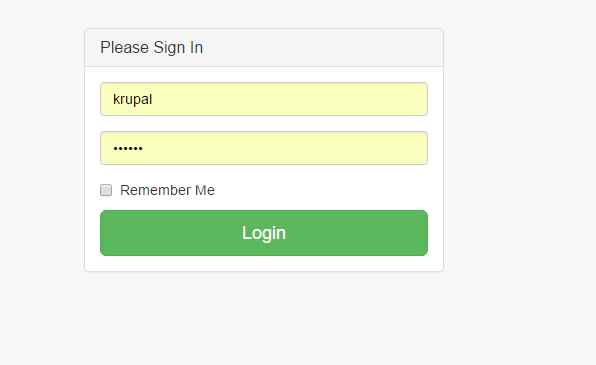
\includegraphics[scale=1]{project/11}\hspace*{\fill}
    \caption{Login}
    \label{f1}
\end{minipage}        
\end{figure}  

\begin{figure}[!h]
\begin{minipage}[t]{0.5\linewidth}
    \centering
\hfill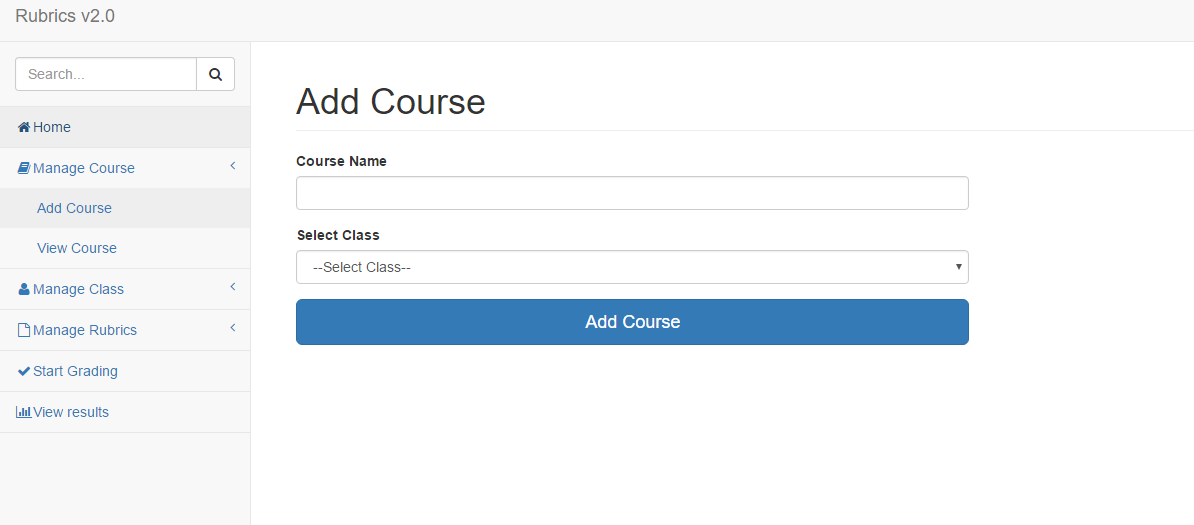
\includegraphics[width=17cm, height=11cm]{project/12}\hspace*{\fill}
    \caption{Add Course}
    \label{f1}
\end{minipage}        
\end{figure} 

\begin{figure}[!h]
\begin{minipage}[t]{0.5\linewidth}
    \centering
\hfill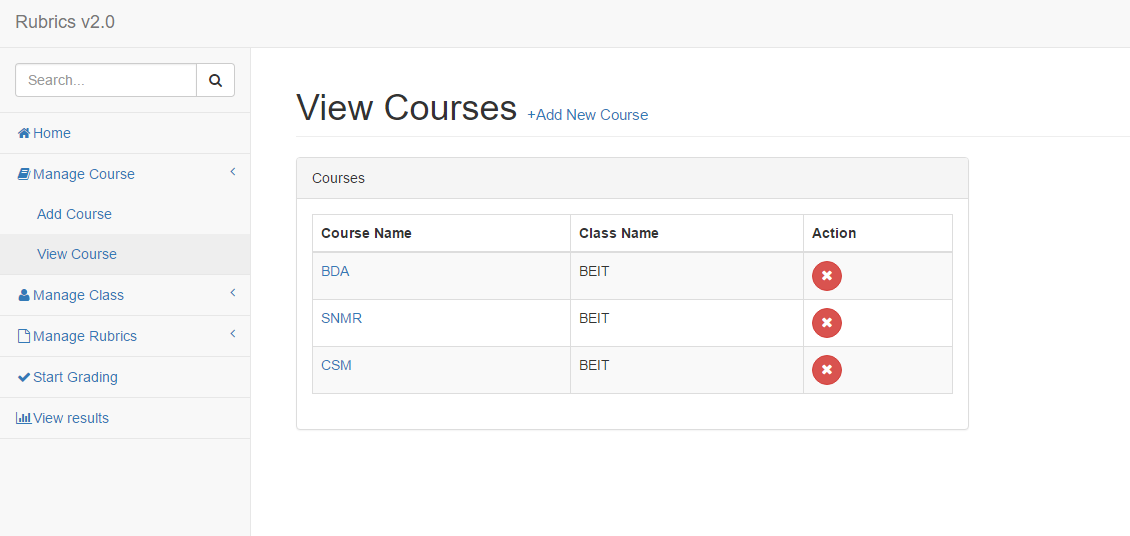
\includegraphics[width=17cm, height=11cm]{project/13}\hspace*{\fill}
    \caption{View Course}
    \label{f1}
\end{minipage}        
\end{figure}

\begin{figure}[!h]

\begin{minipage}[t]{0.5\linewidth}
    \centering
\hfill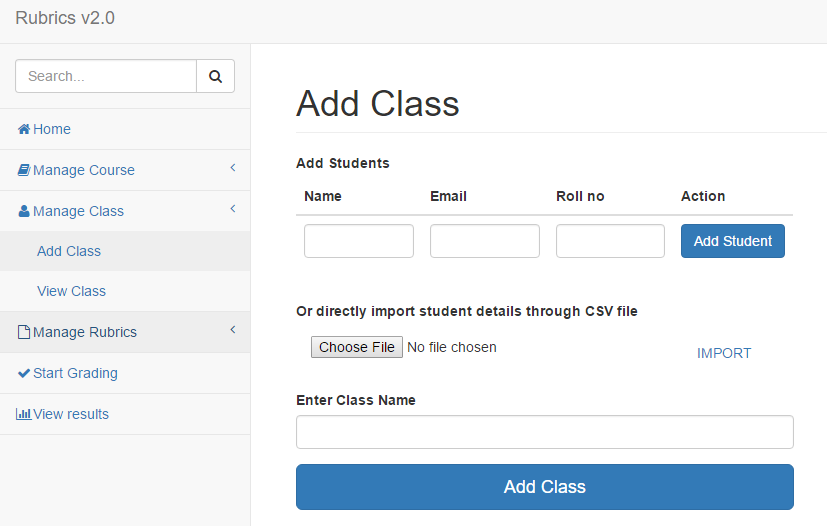
\includegraphics[width=17cm, height=12cm]{project/14}\hspace*{\fill}
    \caption{Add Class}
    \label{f1}
\end{minipage}        
\end{figure}

\begin{figure}[!h]
\begin{minipage}[t]{0.5\linewidth}
    \centering
\hfill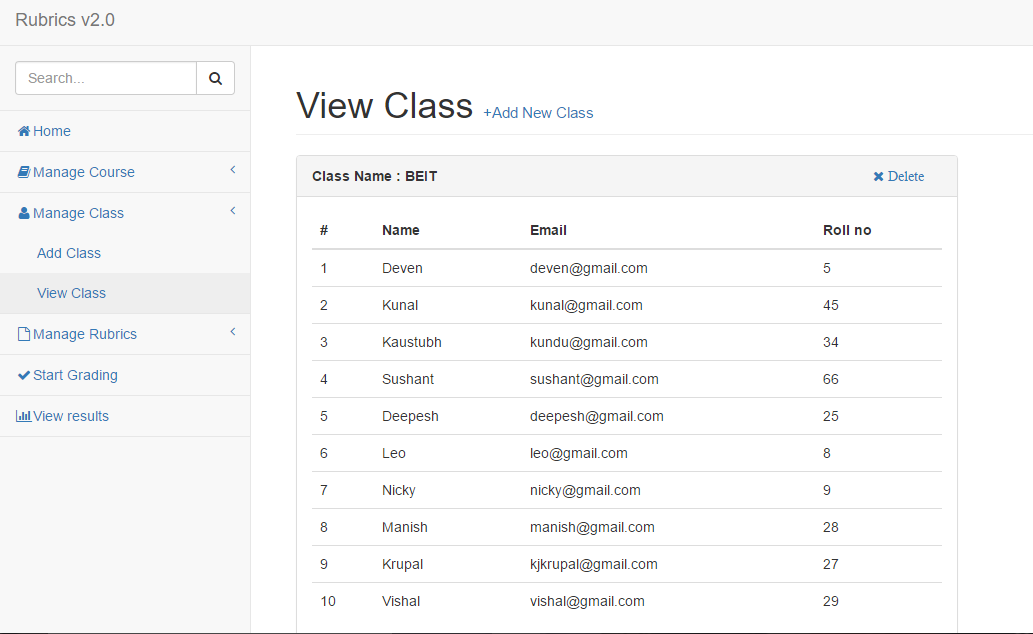
\includegraphics[width=17cm, height=11cm]{project/15}\hspace*{\fill}
    \caption{View Class}
    \label{f1}
\end{minipage}        
\end{figure}

\newpage

\section{Testing}
\vspace{-0.5cm}
Testing process constitutes checking errors in the code. The main objective of testing is to find the undiscovered errors in the code.\\
There are various methods of testing the code \\
\textbf{White Box Testing:}
To check the control structure of the program White box Testing can be used.
Test cases ensure that all the nationalities of the software have been tested at least once.\\
\textbf{Black Box Testing:}
Black box testing is designed to check if the software validations are properly done without considering the internal working of the software.\\
\textbf{Unit Testing:}
In Unit testing all the modules of the software are tested to check if they are in accordance with the modules provided during the design phase. Testing the internal logic of the code is the main motive of Unit testing. White box testing techniques are utilized to check if the control structure is good and does maximum error detection.

\subsection{Test Cases}
Test cases for Modules / component \\
\begin{figure}[H]
\centering
\hfill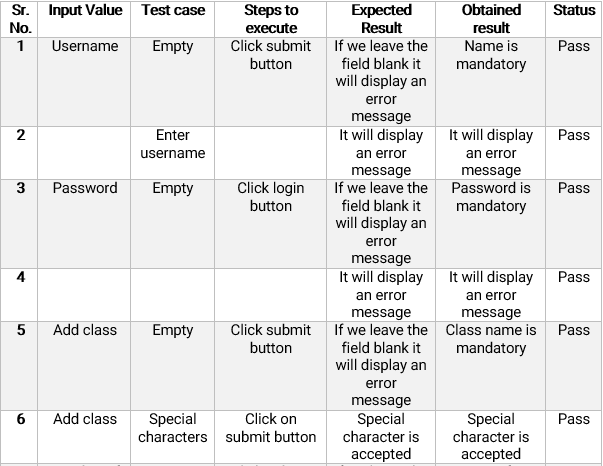
\includegraphics[scale=0.9]{project/images/test1}\hspace*{\fill}
\caption{Test case 1}
\end{figure}

\begin{figure}[H]
\centering
\hfill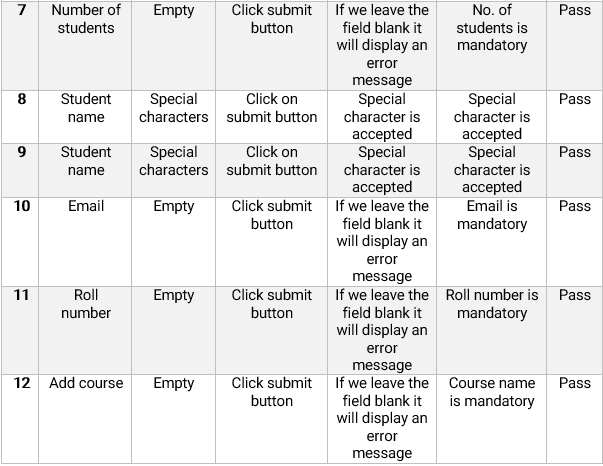
\includegraphics[scale=0.9]{project/images/test2}\hspace*{\fill}
\caption{Test case 2}
\end{figure}

\begin{figure}[H]
\centering
\hfill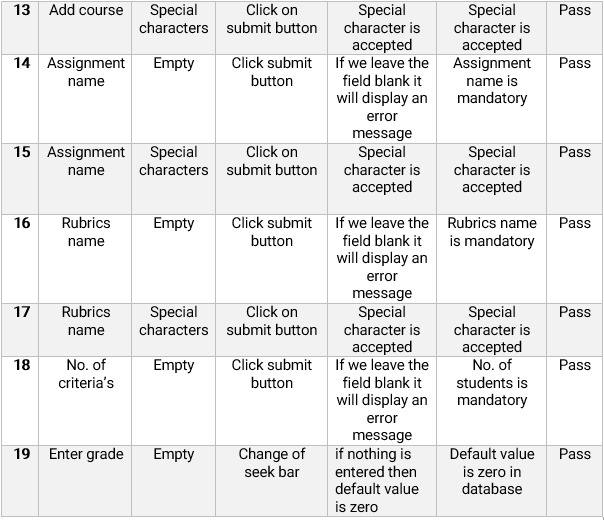
\includegraphics[scale=0.9]{project/images/test3}\hspace*{\fill}
\caption{Test case 3}
\end{figure}